\documentclass[a4paper]{article}
\usepackage[utf8]{inputenc}
\usepackage[russian,english]{babel}
\usepackage[T2A]{fontenc}
\usepackage[left=10mm, top=20mm, right=18mm, bottom=15mm, footskip=10mm]{geometry}
\usepackage{indentfirst}
\usepackage{amsmath,amssymb}
\usepackage[italicdiff]{physics}
\usepackage{graphicx}
\graphicspath{{images/}}
\DeclareGraphicsExtensions{.pdf,.png,.jpg}
\usepackage{wrapfig}

\usepackage{caption}
\captionsetup[figure]{name=Рисунок}
\captionsetup[table]{name=Таблица}
  
\title{\underline{Отчет о выполненой лабораторной работе 1.3.2}}
\author{Воронин Денис, Б04-403}


\begin{document}

\maketitle
\begin{center}
    \Large{\textbf{Определение модуля кручения статестическим и динамичечким методами}}
\end{center}


\section{Aннотация}
\textbf{Цель работы: }измерение углов закручивания в зависимости от приложенного момента
сил, определение модулей для проволки по измерениям периодов крутильных колебаний подвешенного на
ней маятника\par
\textbf{Оборудование: }проволка из исследуемого материала,
грузы, секундомер, микрометр, рулетка, линйка.
\section{Теоретические сведения}
При закручивании цилиндрических стержней круглого сечения распределение деформаций
 и напряжений одинаково по длине стержня только вдали от мест, где прикладываются закручивающие моменты.
Для этих областей можно считать, что каждое поперечное сечение поворачивается поворачивается как жествкое,
то есть частички материала не сходят с радиальных линий, на которых они были в начале, и все
эти линии поворачиваются на один и тот же угол. Такое напряженное состояние назвается чистым кручением.\\

При такой деформации любая прямая линия, проведенная до закручивания цилиндра по частицам материала и параллельная оси симметрии,
при закручивании превращается в спираль(винтовую линию).

Если к стержню приложить закручивающий момент M, то конец стерржня повернется на угол $\varphi$ , причем, согласно закону Гука
\[M= f\varphi (1)\]
Постоянная величина $f$ носит название модуля кручения. Модуль кручения связан с модулем сдвига матнриала стержня $G$ соотношением 
\[f = \frac{\pi G \rho^4}{2L}(2)\]
где $\rho $ -радиес, а L- длина стержня

\section{Установка}
\begin{wrapfigure}{l}{0.5\textwidth}
    \centering
    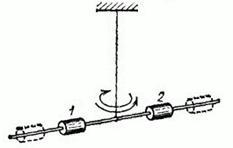
\includegraphics[width=0.4\textwidth]{pick1.jpg}
\end{wrapfigure}
Верхний конец проволоки зажат в цангу и при помощи специального приспособления поворачивается вместе с цангой вокруг вертикальной оси. Запишем для этого случая уравнение движения:
\[M = I\frac{d^2\varphi }{dt^2}(3)\] 
Здесь M - момент сил, I - момент инерции стержня с грузами, $\varphi $- угол поворота стержня. \par
После подстановки (1) формула (3) приобретает вид:
\[\frac{d^2\varphi }{dt^2} + \omega^2\varphi = 0, \omega^2 = \frac{f}{I}(4)\] 
Отсюда 
\[\varphi = \varphi_{0}\sin(\omega t+\theta )(5)\]
где амплитуда $\varphi_{0}$ и начальная фаза  $\vartheta $ определяются начальными условиями.\par
Период крутильных колебаний стержня равен
\[T = \frac{2\pi }{\omega } =2\pi \frac{I}{f}\]  

\section{Ход работы}
Установим диапазон амлитуд при котором T = const\par
Установив грузы так,чтобы их центры масс находились на некотором расстоянии $L_{1}$ от оси системы измерим период.
Если I - момент инерции без грузов, а $I_{1}$ - момент инерции грузо, то очевидно,
\[T_{1} = 2\pi \sqrt{\frac{I+I_{1}}{f} }(6)\]
Изменив расстояние грузов до величины $L_{2}$ получим
\[T_{2} = 2\pi \sqrt{\frac{I+I_{2}}{f} }(7)\]
Из (6) и (7) следует 
\[f=\frac{4\pi^2(I_{1}-I_{2})}{T_{1}^2-T_{2}^2 }= \frac{8\pi^2m(L_{1}^2-L_{2}^2)}{T_{1}^2-T_{2}^2} \]
По результатам измерений имеем

\begin{table}[!h]
    \begin{center}
    \begin{tabular}{|l|l|l|l|l|}
    \hline
    $L_{1}$ cm &$L_{2}$ cm& $T_{1}$& $T_{2}$& f \\ \hline
    13,5& 6,75& 39,5& 22,1& $7,5*10^{-4}$ \\ \hline
    12,5& 6,25& 37,1& 21,4& $7,54*10^{-4}$ \\ \hline
    11,5& 5,75& 34,5& 20,0& $7,51*10^{-4}$ \\ \hline
    10,5& 5,25& 32,0& 19,0& $7,53*10^{-4}$ \\ \hline
\end{tabular}
\caption{Результаты измерений}
\end{center}
\end{table}
Отсюда среднее значение f будет равно $f= 7,52*10^{-4} \frac{\text{кг}*\text{м}^{2}}{c^2}$\par
Найдем модуль сдвига G по формуле 
\[G = \frac{2l_{0}f}{\pi R^{4}}(8) = \frac{2*17,50*7,52*10^{-4}}{\pi *0,001^{4}} = 8,4*10^{9} \frac{\text{Н}}{\text{м}^{2}} \]
Для оценок погрешностей воспользуемся формулами
\[\sigma_{f}= f\sqrt{(\frac{\sigma_{m}}{m})^{2} + (\frac{\sigma_{l}}{l} )^{2}+(\frac{\sigma_{T}}{T} )^2} = 0,033*10^{-2}\] 
\[\sigma_{G}= f\sqrt{(\frac{\sigma_{l_{0}}}{l})^{2} + (\frac{\sigma_{f}}{f} )^{2}+(\frac{4\sigma_{R}}{R} )^2} = 0,15*10^{9}\]
В конечном итоге имеем $G =42*10^{9}\pm 0,15*10^{9} \frac{\text{Н}}{\text{м}^{2}} $ 
\newpage
\section{Вычисление G статическим методом}
\begin{wrapfigure}{l}{0.5\textwidth}
    \centering
    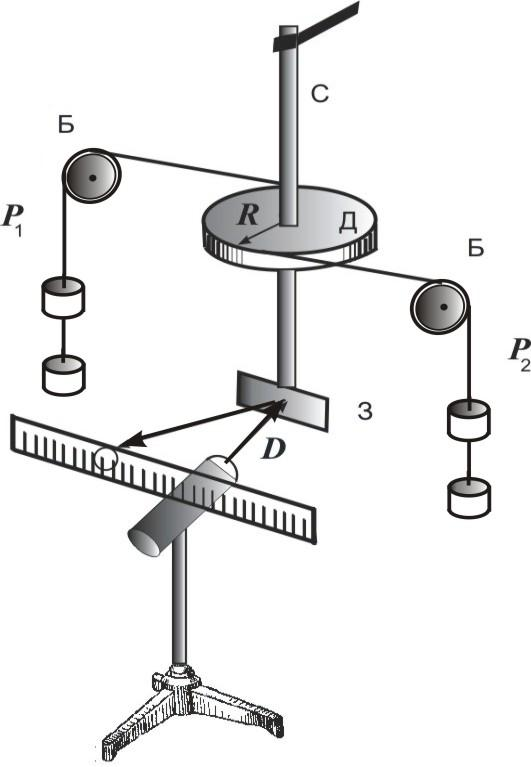
\includegraphics[width=0.23\textwidth]{pick2.jpg}
\end{wrapfigure}
Схема экспериментальной установки для статического закручивания стержня изображена на рис. 2. Верхний конец вертикально расположенного стержня  жестко закреплен на стойке, а нижний соединен
с диском. Момент М, закручивающий стержень, создают две навитые на диск и перекинутые через блоки Б нити, к концам которыхподвешиваются одинаковые грузы Г. Диск снабжен зеркальцем 3. Для
определения угла закручивания стержня надо зрительную трубу направить на зеркальце и добиться того, чтобы в нее было четко видно
отражение шкалы, укрепленной на том же штативе, что и труба. Измерение смещения изображения шкалы в трубе позволяет определить
угол закручивания стержня.\par
Параметры установки: l = 170 см диаметр стержня 2 мм, радиус диска 7 см

\begin{table}[!h]
    \begin{center}
    \begin{tabular}{|l|l|l|l|l|l|}
    \hline
    m,г &$\downarrow $,см& $\uparrow $, см& $\bigtriangleup l$ см& M, Н*м& 2$\varphi $ \\ \hline
    100& 3& 3,1& 3,05& 0,14& 1,03 \\ \hline
    200& 5,9& 5,7& 5,8& 0,28& 1,95 \\ \hline
    400& 11,8& 11,9& 11,85& 0,56& 3,98 \\ \hline
    600& 18& 18,2& 18,1& 0,84& 6,01 \\ \hline
    700& 19,8& 21,0& 20,4& 0,98& 6,84 \\ \hline
    800& 23,9& 23,9& 23,9& 1,12& 8,00 \\ \hline
\end{tabular}
\caption{Результаты измерений}
\end{center}
\end{table}

Построим график в координатах $\varphi (M)$:
\begin{figure}[h]
    \centering
    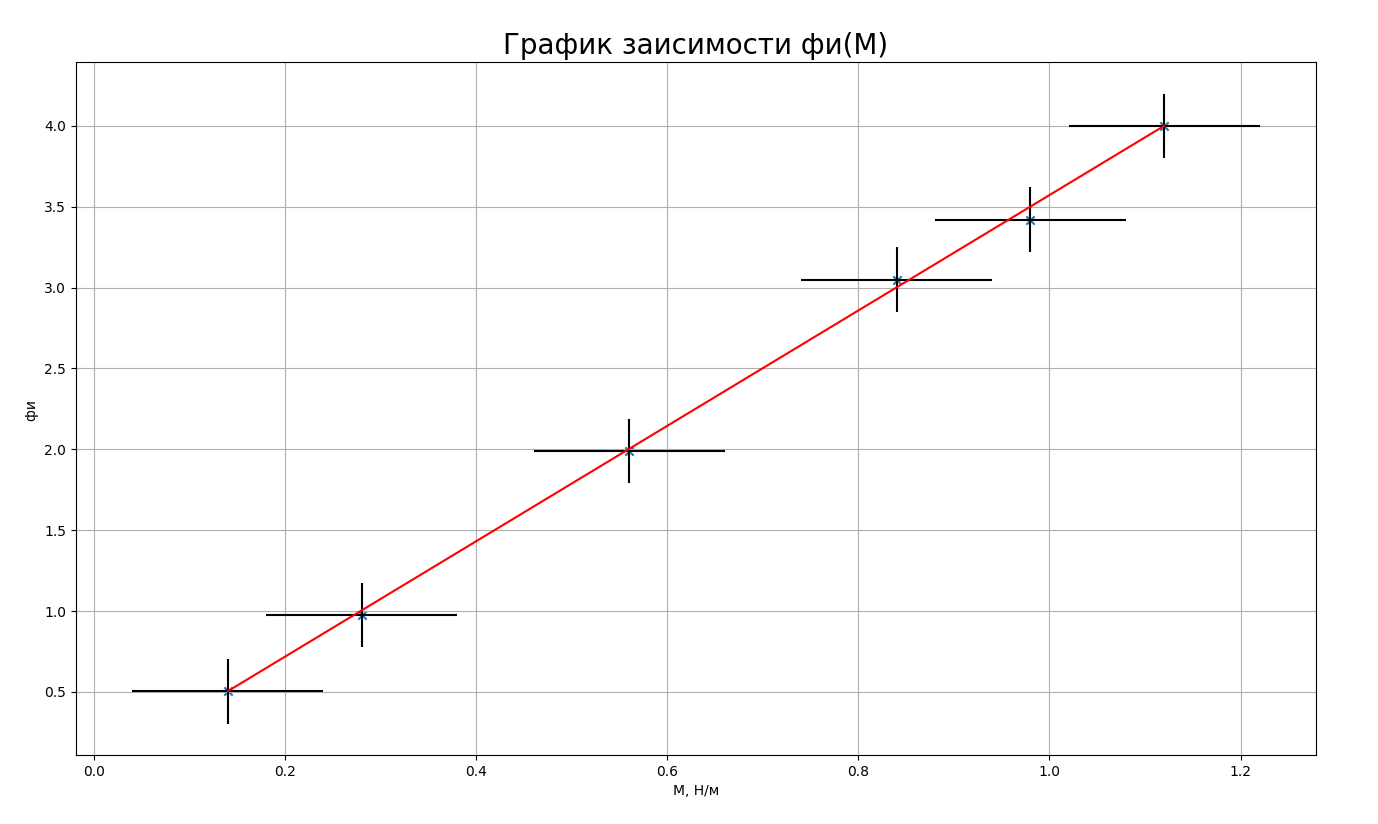
\includegraphics[width=1\textwidth]{pick3.PNG} 
    \caption{График $\varphi(M)$}
    \end{figure}
Откуда $f= 3,56*10^{-4} \frac{\text{кг}*\text{м}^{3}}{c^{2}}$\par
Используя формулу (8) найдем модуль сдвига: $G = 4*10^{9} \frac{H}{\text{м}^{2}} $
\end{document}